\section{Filter}\label{sec:filter_design}

The aim of this chapter is to analyse the data from \ref{sec:opt_result} and choose the implementation method. From the beam forming optimization \autoref{sec:genetic_con} it was concluded that there shall be a cost filter and a beam forming filter. This chapter starts analyse the cost filter and design a filter solution, then the beam forming filter will be analysed and a solution will be designed.


\section{The cost filter}
The analysis of the cost filter will be done only with respect to the gain of the transfer function and without taking the phase intro account. The reason to avoid the phase is that the filter is an input filter to the entire system, and therefore the phase of the filter will affect all speaker the same way and therefore not effect the beam forming. \\
To analyse the cost filter, the filter type and the slope or Q of the filter have to be determined. 

the filter type will be determined first. To determined the filter type, a second order polynomia estimation will be done on the data point of the cost filter. The polynomia estimation is done with MATLAB command \texttt{polyfit()} with a second order regression. This give a second order polinomia where  \texttt{polyval()} is used to estimate the filter transfer function. The estimation will be done from \SI{60}{\hertz} to \SI{400}{\hertz}. The \SI{400}{\hertz} choice is made such that the estimation fit at lest to the double frequency of beam forming interest. The following \autoref{} shows the estimate compare to the original data point.

\begin{figure}[H]
	\centering
	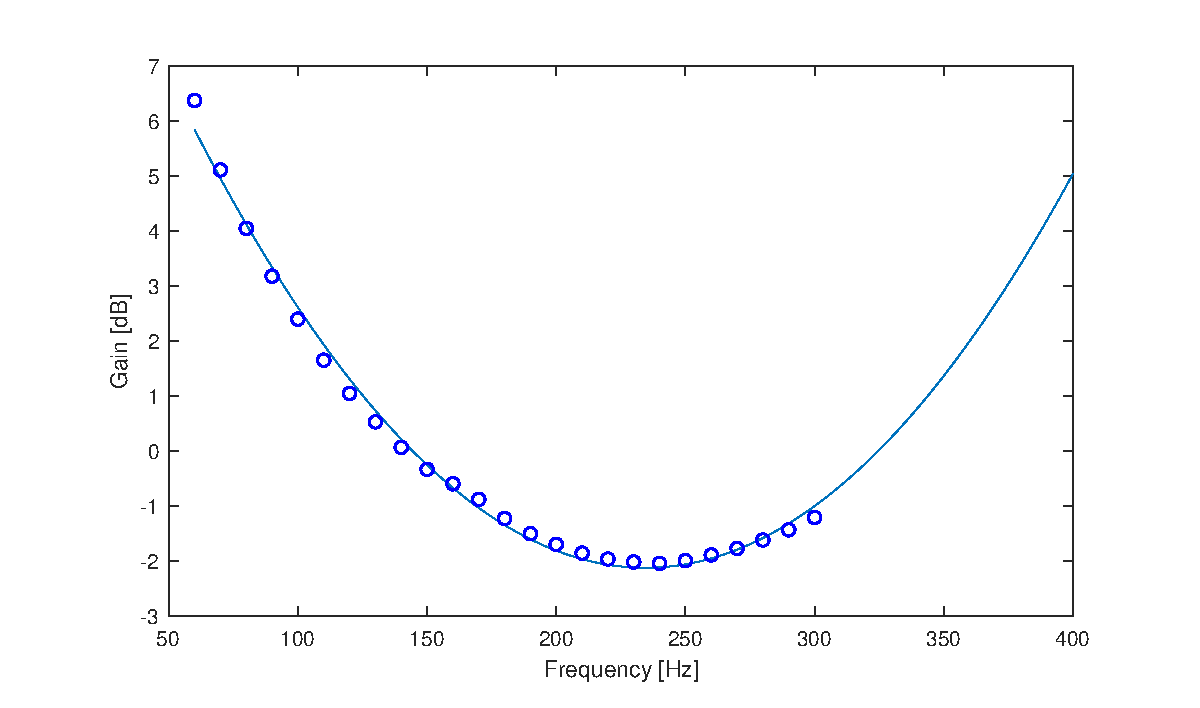
\includegraphics[width=1\textwidth]{band_stop_filter.eps}
	\caption{The graph shows transfer function of the estimated transfer function, where the blue  Solid line is the gain. All circle in the graph is the actual optimized point.}
		\label{fig:band_stop_filter}
\end{figure}
It can also be seen on \autoref{band_stop_filter} the shape of the estimated cost filter is a band stop filter. \\

\subsection{Parametric equalizer as cost filter}

Designing a bandstop filter is done with designing it as a bandpass filter, and use it in a feedback circuit. The following block diagram \autoref{fig:bandstop_filter_blockdiagram} shows a block diagram of a bandstop filter. 

\begin{figure}[H]
	\centering
\begin{picture}(0,0)%
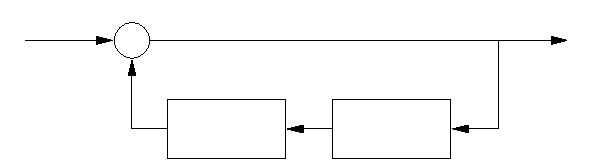
\includegraphics{bandstop_filter_blockdiagram.pdf}%
\end{picture}%
\setlength{\unitlength}{4144sp}%
%
\begingroup\makeatletter\ifx\SetFigFont\undefined%
\gdef\SetFigFont#1#2#3#4#5{%
  \reset@font\fontsize{#1}{#2pt}%
  \fontfamily{#3}\fontseries{#4}\fontshape{#5}%
  \selectfont}%
\fi\endgroup%
\begin{picture}(4634,1218)(2056,-973)
\put(2071, 74){Input}%
\put(3196,-376){-}%
\put(3556,-781){Gain}%
\put(4681,-781){Bandpass}%
\put(2791,-286){+}%
\put(6076, 74){Output}%
\end{picture}%
	\caption{The figure shows the block diagram of a bandstop filter}
		\label{fig:bandstop_filter_blockdiagram}
\end{figure}


Designing the bandpass filter part of the bandstop filter, the bandpass filter part is changed such that the center frequency is at \SI{0}{\decibel} and the shape is a bandpass filter and not a bandstop filter. To change the filter, the parameter is inverter and subtracted \SI{2.1}{\decibel}. The following \autoref{fig:band_pass_filter} shows the bandpass filter.

\begin{figure}[H]
	\centering
	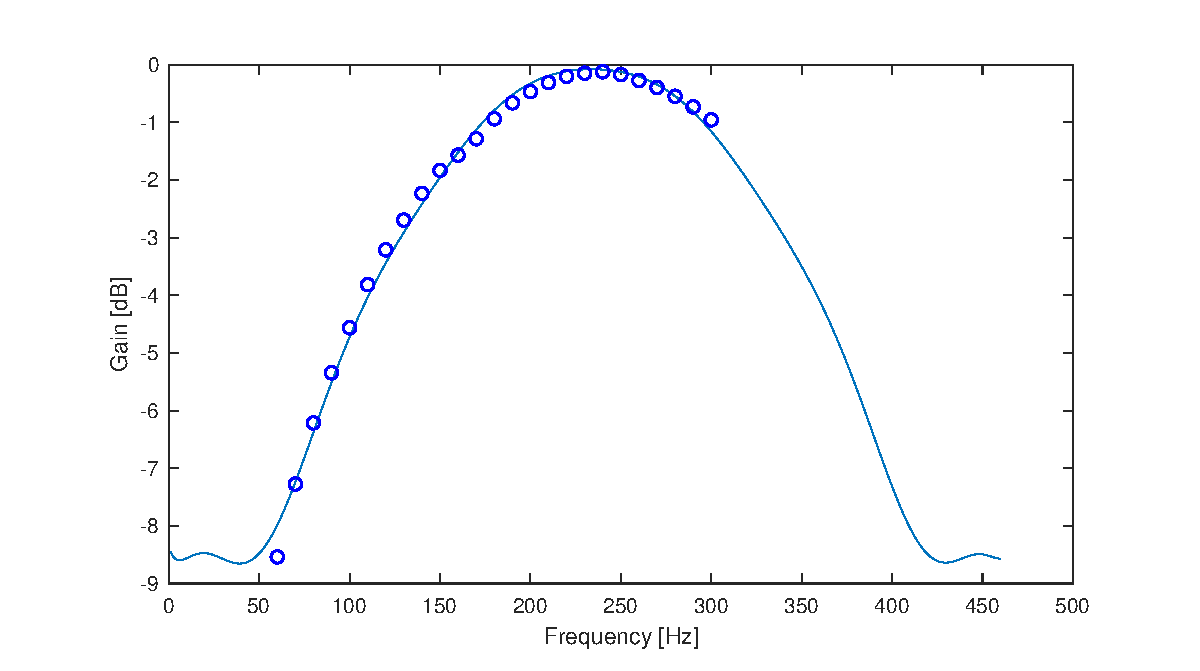
\includegraphics[width=1\textwidth]{band_pass_filter.eps}
	\caption{The graph shows transfer function of the estimated transfer function, where the blue  Solid line is the gain. All circle in the graph is the actual optimized point.}
		\label{fig:band_pass_filter}
\end{figure}

On \autoref{fig:band_pass_filter} it can be seen that the \SI{-3}{\decibel} bandwidth is \SI{293}{\hertz} with a relative gain of \SI{8.5}{\decibel}, and have a center frequency of \SI{234}{\hertz}. There needs to be a gain factor before the filter, to achieve the wanted band stop filter. The initial filter parameters is then:

\begin{itemize}
\item Gain $G = \SI{8.5}{\decibel}$
\item Bandwidth is $BW = 2\pi \SI{293}{\hertz} = 1841$
\item Center frequency is $\omega_0 = 2\pi \SI{234}{\hertz} = 1470.3$
\item The filter goodness $Q = \frac{1470.3}{1841} = 0.7986$
\end{itemize}

The corresponding transfer function to block diagram \autoref{fig:bandstop_filter_blockdiagram} is as \autoref{eq:bandstop_filter_eq}

\begin{equation}\label{eq:bandstop_filter_eq}
H_{stop}(s) = \frac{s^2+\frac{\omega_0}{Q}s+\omega_0^2}{s^2+\frac{\omega_0}{Q}s(1+Gain)+\omega_0^2}
\end{equation}

A bode plot of the \autoref{eq:bandstop_filter_eq} is showen in \autoref{fig:bandstop_filter_eq_bodeplot}



\begin{figure}[H]
	\centering
	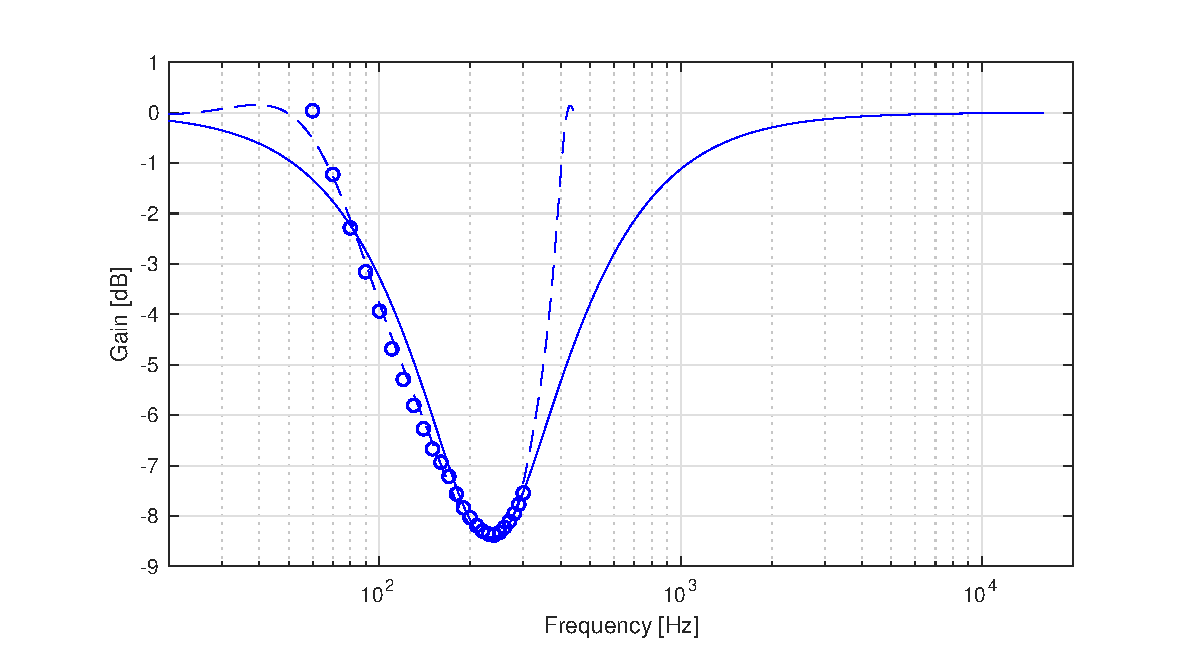
\includegraphics[width=1\textwidth]{bandstop_filter_eq_bodeplot.eps}
	\caption{The figure shows the bode plot of the \autoref{{eq:bandstop_filter_eq}}}
		\label{fig:bandstop_filter_eq_bodeplot}
\end{figure}

On the bode plot  \autoref{fig:bandstop_filter_eq_bodeplot} the filter parameter fits well from \SI{100}{\hertz} and upwards but the frequency that is below \SI{100}{\hertz} is to fare off. To solve this problem, the data point can be attenuated to fit on the steep slop of the filter. Therefore the data point is attenuated by \SI{4}{\decibel} and as wall as the filter. The following \autoref{fig:bandstop_filter_eq_bodeplot_attenuated} shows the result.

\begin{figure}[H]
	\centering
	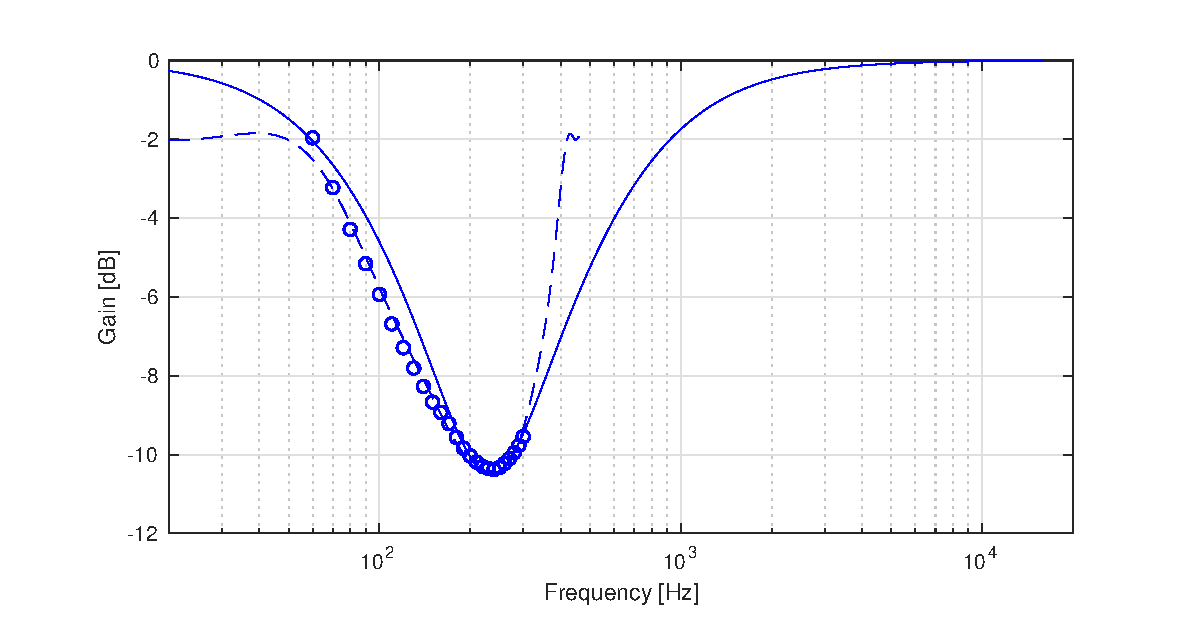
\includegraphics[width=1\textwidth]{bandstop_filter_eq_bodeplot_attenuated.eps}
	\caption{The figure shows the bode plot of the \autoref{{eq:bandstop_filter_eq}}}
		\label{fig:bandstop_filter_eq_bodeplot_attenuated}
\end{figure}


As it can be seen on \autoref{fig:bandstop_filter_eq_bodeplot_attenuated} that the change have affacted the fit positive. The filter gain is therefore changed to  $G = \SI{12.5}{\decibel}$ in the parameters. Recalling from \autoref{fig:bandstop_filter_eq_bodeplot_attenuated} the filter is attenuated with \SI{4}{\decibel} and therefore the front gain which i called $\test{In_Gain}$ shall be amplified by \SI{4}{\decibel} plus the \SI{6.4}{\decibel} which correspond to the inverting in \autoref{fig:band_pass_filter}. The gain in front of the cost filter then have to be \SI{10.4}{\decibel}. The corresponding block diagram for the filter including the gain in front of the filter is as \autoref{fig:bandstop_filter_blockdiagram_gain}

\begin{figure}[H]
	\centering
\begin{picture}(0,0)%
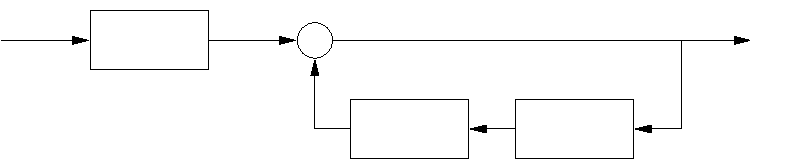
\includegraphics{bandstop_filter_blockdiagram_gain.pdf}%
\end{picture}%
\setlength{\unitlength}{4144sp}%
%
\begingroup\makeatletter\ifx\SetFigFont\undefined%
\gdef\SetFigFont#1#2#3#4#5{%
  \reset@font\fontsize{#1}{#2pt}%
  \fontfamily{#3}\fontseries{#4}\fontshape{#5}%
  \selectfont}%
\fi\endgroup%
\begin{picture}(6029,1218)(661,-973)
\put(1486,-106){In_Gain}%
\put(3196,-376){-}%
\put(3556,-781){Gain}%
\put(4681,-781){Bandpass}%
\put(2791,-286){+}%
\put(6076, 74){Output}%
\put(676, 74){Input}%
\end{picture}%
	\caption{The figure shows the block diagram of a bandstop filter}
		\label{fig:bandstop_filter_blockdiagram_gain}
\end{figure}

\begin{equation}\label{eq:bandstop_filter_eq_analogue}
H_{stop}(s) = \text{In_Gain} \cdot \frac{s^2+\frac{\omega_0}{Q}s+\omega_0^2}{s^2+\frac{\omega_0}{Q}s(1+Gain)+\omega_0^2}
\end{equation}

The corresponding cost filter to the transfer function \autoref{eq:bandstop_filter_eq_analogue} is \autoref{fig:cost_filter_final}

\begin{figure}[H]
	\centering
	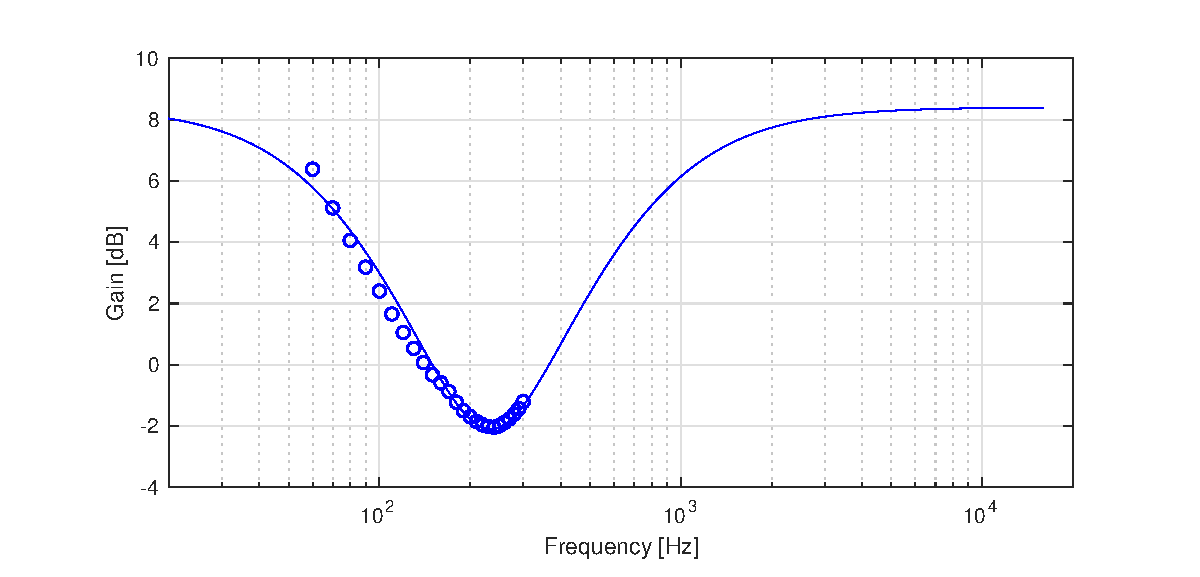
\includegraphics[width=1\textwidth]{cost_filter_final.eps}
	\caption{The figure shows the bode plot of the block diagram \autoref{fig:bandstop_filter_blockdiagram_gain}}
		\label{fig:cost_filter_final}
\end{figure}


The transfer function for for the filter is then \autoref{eq:bandstop_filter_eq_analogue}



\subsection{Converting the cost filter to differential equation}
In order to implement the cost filter in MATLAB to generate the filtered sine swept, the analogue designed filter has to be converted to a digital filter. The conversion will be made by using the bilinear transformation, which convert analogue filter intro \gls{iir} filter.  The transformation is done by changing the s in \autoref{eq:bandstop_filter_eq_analogue}, the bilinear transformation is as following 

\begin{equation}\label{eq:bandstop_filter_bilinear}
H_{stop}(z) = H_{stop}(s) \mid_{s=\frac{2}{T_s}\frac{z-1}{z+1}} 
\end{equation}

    \startexplain
        \explain{$H(z)$ is the digital transfer function}{1}
        \explain{$T_s$ is the sample time}{\si{\second}}
    \stopexplain

By applying the conversion \autoref{eq:bandstop_filter_bilinear} to the analogue cost filter, the filter become \autoref{eq:bandstop_filter_eq_z}

\begin{equation}\label{eq:bandstop_filter_eq_z}
H_{stop}(s) = \text{In_Gain} \cdot \frac{(\frac{2}{T_s}\frac{z-1}{z+1})^2+\frac{\omega_0}{Q}\frac{2}{T_s}\frac{z-1}{z+1}+\omega_0^2}{(\frac{2}{T_s}\frac{z-1}{z+1})^2+\frac{\omega_0}{Q}\frac{2}{T_s}\frac{z-1}{z+1}(1+Gain)+\omega_0^2}
\end{equation}

The \autoref{eq:bandstop_filter_eq_z} is changed such that all fixed values is changed to a- end b coefficient. The following \autoref{eq:bandstop_filter_peak_att} is the digital transfer function.


\begin{equation}\label{eq:bandstop_filter_peak_att}
        H_{stop}(z) =  \text{In_Gain} \cdot \frac{z^2 \cdot a_{stop1} + z \cdot a_{stop2} + a_{stop3}}{z^2 \cdot b_{stop1} + z \cdot b_{stop2} + b_{stop3}}
    \end{equation}
    
    \startexplain
     \explain{$H_{stop}(z)$ is the digital transferfunction for the attenuating peak filter.}{\si{1}}
     \explain{$b_{stop1} = 4 \cdot Q + \omega_0 \cdot(1+G) \cdot T_s \cdot 2 + \omega_0^2 \cdot T_s^2 \cdot Q  $ }{\si{1}}
     \explain{$b_{stop2} =-8 \cdot Q + 2 \cdot  \omega_0^2 \cdot T_s^2 \cdot Q$ }{\si{1}}
     \explain{$b_{stop3} = 4 \cdot Q - 2 \cdot \omega_0 \cdot T_s \cdot (1+G) + \omega_0^2 \cdot T_s^2 \cdot Q$ }{\si{1}}
     \explain{$a_{stop1} = 4 \cdot Q + 2 \cdot \omega_0 \cdot T_s + \omega_0^2 \cdot T_s^2 \cdot Q$ }{\si{1}}
     \explain{$a_{stop2} = -8 \cdot Q + 2 \cdot  \omega_0^2 \cdot T_s^2 \cdot Q$ }{\si{1}}
     \explain{$a_{stop3} = 4 \cdot Q - 2 \cdot \omega_0 \cdot T_s + \omega_0^2 \cdot T_s^2 \cdot Q$ }{\si{1}}
    \stopexplain

The last step is to convert the cost filter from z-Domain to transfer function intro differential equation in discrete time domain "n". The following step in \autoref{} is doing the domain conversion.



\begin{subequations}\label{eq:bandstop_filter_peak_n}
\begin{alignat}{2}
 H_{stop}(z)=\frac{Y(z)}{X(z)} &=  \text{In_Gain} \cdot \frac{z^2 \cdot a_{stop1} + z \cdot a_{stop2} + a_{stop3}}{z^2 \cdot b_{stop1} + z \cdot b_{stop2} + b_{stop3}} \label{eq:bandstop_filter_peak_n_1}\\
 H_{stop}(z)=\frac{Y(z)}{X(z)} &=  \text{In_Gain} \cdot \frac{a_{stop1} + z^{-1} \cdot a_{stop2} +  z^{-2} \cdot a_{stop3}}{b_{stop1} + z^{-1} \cdot b_{stop2} +  z^{-2} \cdot b_{stop3}}  \label{eq:bandstop_filter_peak_n_2}
\end{alignat}
\end{subequations}


\begin{subequations}
    \centering
$\Updownarrow$
\begin{equation}\label{eq:z_to_n3}
        Y(z) \cdot (b_{stop1} + b_{stop2} \cdot z^{-1} + b_{stop3} \cdot z^{-2}) = X(z) \cdot \text{In_Gain} \cdot (a_{stop1} + a_{stop2} \cdot z^{-1} + a_{stop3} \cdot z^{-2})
    \end{equation}
       \centering
$\Updownarrow$
\begin{equation}\label{eq:z_to_n4}
         Y(z) \cdot b_{stop} + Y(z) \cdot b_{stop2} \cdot z^{-1} + Y(z) \cdot b_{stop3} \cdot z^{-2} =  \text{In_Gain} \cdot (X(z) \cdot a_{stop1} + X(z) \cdot a_{stop2} \cdot z^{-1} + a_{stop3} \cdot z^{-2})
    \end{equation}
    \centering
    $\Downarrow Z^{-1}$
\begin{equation}\label{eq:z_to_n5}
         b_{stop1} \cdot y[n] + b_{stop2} \cdot y[n-1] + b_{stop3} \cdot y[n-2] =  \text{In_Gain} \cdot (a_{stop1} \cdot x[n] +  a_{stop2} \cdot x[n-1] + a_{stop3} \cdot x[n-2])
    \end{equation}
    \centering
    $\Updownarrow$
\begin{equation}\label{eq:z_to_n6}
         b_{stop1} \cdot y[n] =  \text{In_Gain} \cdot (a_{stop1} \cdot x[n] + a_{stop2} \cdot x[n-2] + a_{stop3} \cdot x[n-2]) -  b_{stop2} \cdot y[n-1] - b_{stop3} \cdot y[n-2]
    \end{equation}
    \centering
    $\Updownarrow$
\begin{equation}\label{eq:z_to_n7}
         y_{peak}[n] = \frac{\text{In_Gain}  \cdot a_{peak1}}{b_{peak1}} \cdot x[n] + \frac{\text{In_Gain}  \cdot a_{peak2}}{b_{peak1}} \cdot x[n-1] +  \frac{\text{In_Gain}  \cdot a_{peak3}}{b_{peak1}} \cdot x[n-2] -  \frac{b_{peak2}}{b_{peak1}} \cdot y_{peak}[n-1] - \frac{b_{peak3}}{b_{peak1}} \cdot y_{peak}[n-2]
    \end{equation}
    
    \startexplain
     \explain{$y[n]$ is the output sample.}{\si{1}}
     \explain{$x[n]$ is the input sample.}{\si{1}}
    \stopexplain
 \end{subequations}


\section{Beam forming filter}
The beam forming filter is not as easy as the cost filter to design, since that the phase and the gain have to be exact before the beam forming works. Therefore the phase have to be studied to determined the filter type. On the data point from the \ref{sec:opt_result} it can be seen that the phase is mostly linear in the frequency of interest, and therefore the filter will be a linear phase \gls{fir} filter. The smart thing with choosing a \gls{fir} filter is that the impulse response of the filter just have to be symmetric to achieve linear phase response. This means that optimizing the part of the impulse response and put it together with a mirrored version will always achieve linear phase. One disadvantages is that the cut off frequency is in the low frequency and therefore the filter order have to be high. \\

 A modified version of the genetic optimization algorithm will be used to find a optimized impulse response of the filter. To optimize the impulse respond of the filter, an estimate of the impulse respond have to be determined. One and the used way to estimate the impulse response is to transfer all polar coordinate to a complex rectangular transfer function and take the real of the \gls{ifft} of the complex transfer function. The polar to rectangular transform is done as following \autoref{eq:pol_to_regt}

\begin{equation}\label{eq:pol_to_regt}
x=rcos(\phi)+j \cdot rsin(\phi)
\end{equation}


     \startexplain
    \explain{$\phi$ is the angle of the transfer function in radian }{\si{1}}
        \explain{$r$ is the amplitude of the transfer function}{\si{1}}
        \explain{$j$ is the imaginary unit}{\si{1}}
    \stopexplain

The real of the \gls{ifft} gives an estimated impulse response but with a scaled cross over point. The meaning with scaled cross over point is that the cross over point follows the scaling of the sample frequency. With a sample rate of \SI{44.1}{\kilo\hertz} the following  \autoref{} shows the transfer function of the estimated impulse response. 

\begin{figure}[H]
	\centering
	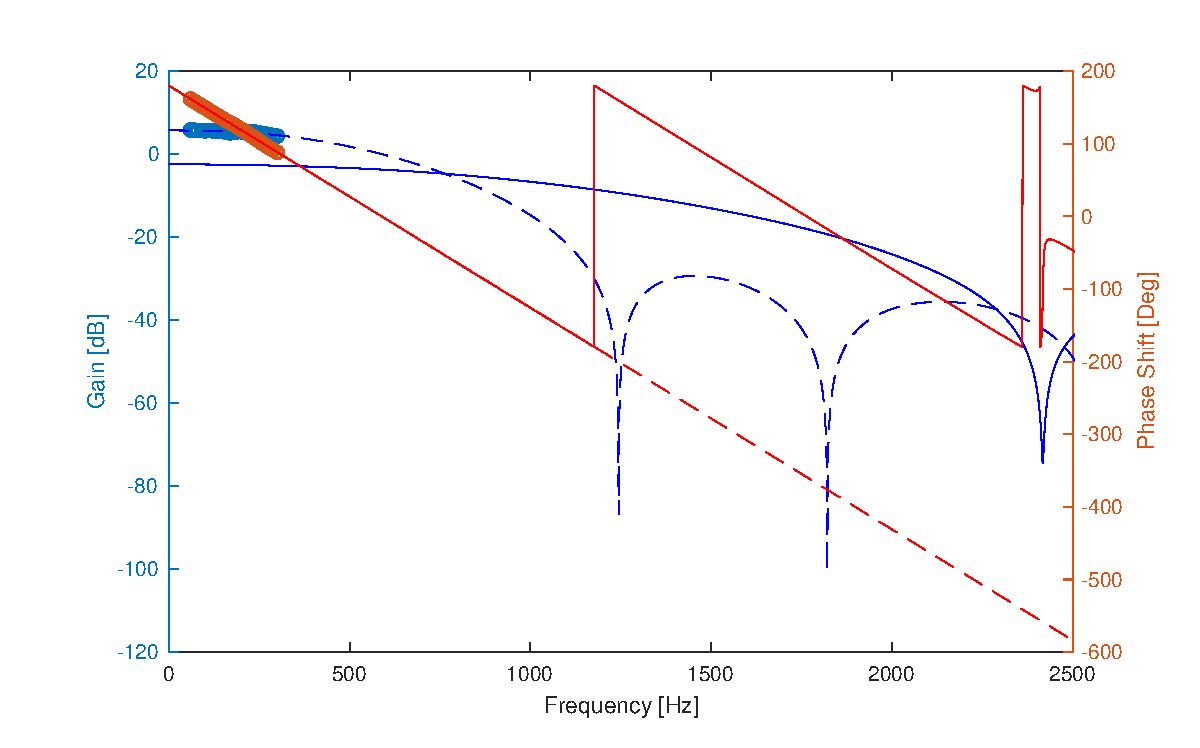
\includegraphics[width=1\textwidth]{ir_estimate_non_scaled.eps}
	\caption{The graph shows transfer function of the estimated impulse respond. The dashed line is transfer function that is needed for beam forming filter, where the blue line is the gain and the red line is the phase. The Solid line line is the transfer function of the estimated impulse response, where the blue line is the gain and the red line is the phase. All circle in the start of the graph is the actual optimized point.}
		\label{fig:ir_estimate_non_scaled}
\end{figure}


It can be seen that the cross over lays at a too high frequency and the gain at the frequency of interest is to low. The corresponding impulse response of the transfer function in \autoref{fig:ir_estimate_non_scaled} is as following \autoref{fig:ir_estimate_non_mirror} where the mirrored version not is added yet. 

\begin{figure}[H]
	\centering
	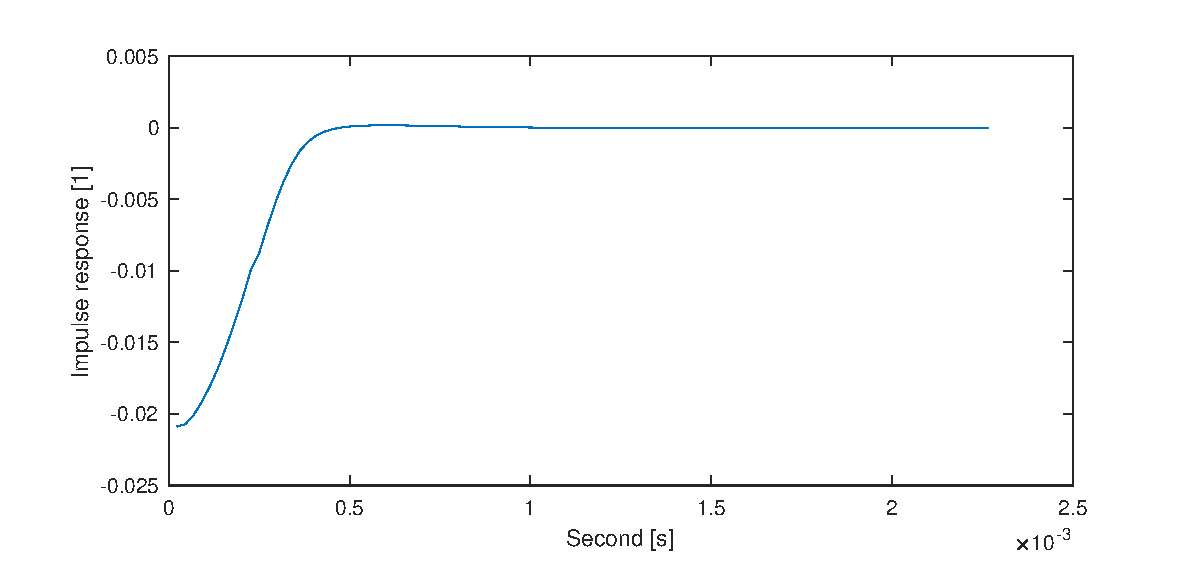
\includegraphics[width=1\textwidth]{ir_estimate_non_mirror.eps}
	\caption{The graph shows the impulse respond where the mirrored version is added to the impulse respond}
		\label{fig:ir_estimate_non_mirror}
\end{figure}

The version where the mirrored impulse response is added to the impulse response and the phase is matched to the wanted phase and is the corresponding impulse response to \autoref{fig:ir_estimate_non_scaled} is \autoref{fig:ir_estimate_mirror}

\begin{figure}[H]
	\centering
	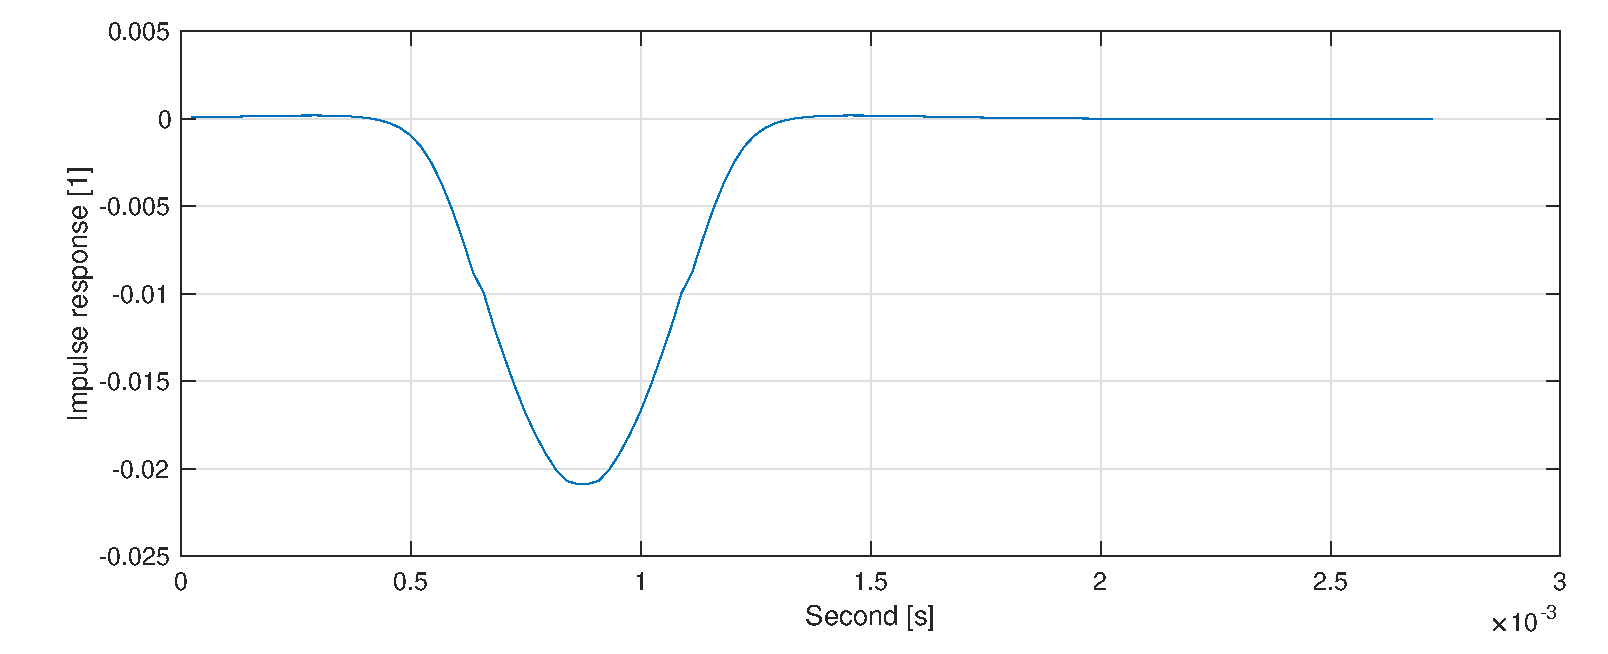
\includegraphics[width=1\textwidth]{ir_estimate_mirror.eps}
	\caption{The graph shows the impulse respond where the mirrored version is added to the impulse respond}
		\label{fig:ir_estimate_mirror}
\end{figure}


The impulse response have to be change the right way to make a good estimate. The way to lower the cross over point is to extend the part of the impulse respond that it have the highest amplitude, which also make the impulse response longer. Thinking about the theory of the \gls{fir} filter, that the lower cross over, the higher order the filter have to be and therefore the impulse respond gets longer. The following \autoref{} shows the estimated impulse respond that will be used for the optimization, where the crossover is approximatly where it shall be. 


\begin{figure}[H]
	\centering
	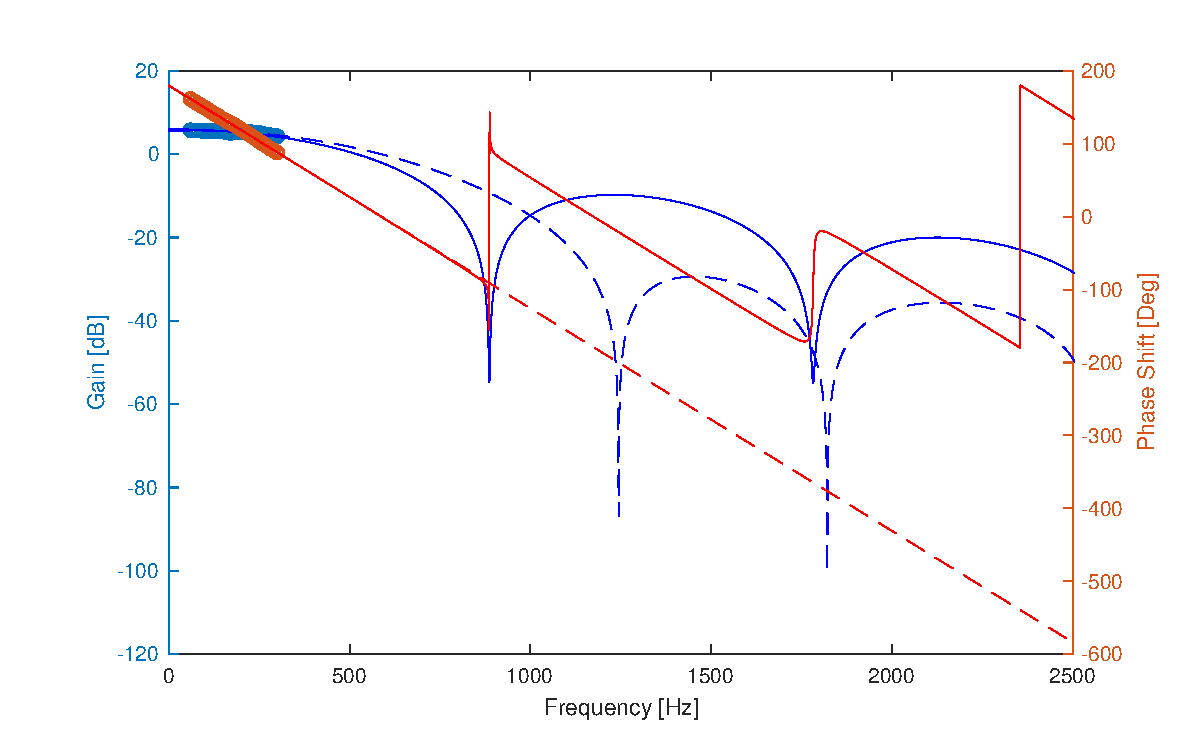
\includegraphics[width=1\textwidth]{ir_estimate_scaled.eps}
	\caption{The graph shows transfer function of the estimated impulse respond. The dashed line is transfer function that is needed for beam forming filter, where the blue line is the gain and the red line is the phase. The Solid line line is the transfer function of the estimated impulse response, where the blue line is the gain and the red line is the phase. All circle in the start of the graph is the actual optimized point.}
		\label{fig:ir_estimate_scaled}
\end{figure}


\begin{figure}[H]
	\centering
	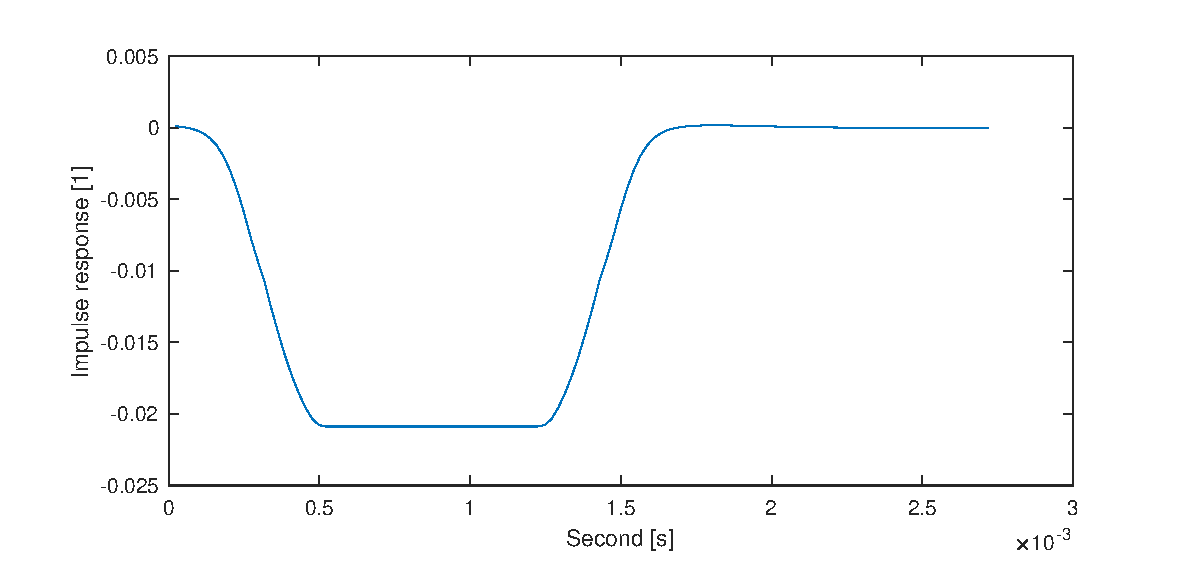
\includegraphics[width=1\textwidth]{ir_estimate_mirror_scale.eps}
	\caption{The graph shows the impulse respond where the mirrored version is added to the impulse respond}
		\label{fig:ir_estimate_mirror_scale}
\end{figure}

Where the corresponding impulse response is as \autoref{fig:ir_estimate_mirror_scale}

\begin{figure}[H]
	\centering
	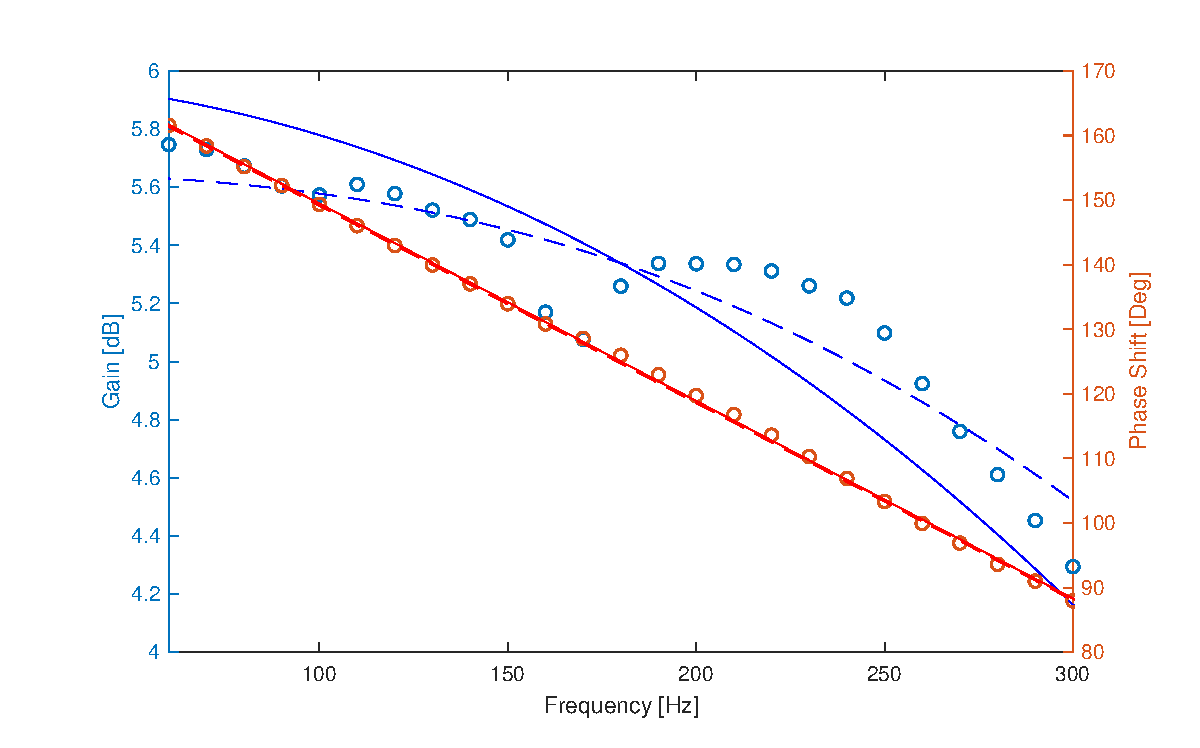
\includegraphics[width=1\textwidth]{ir_estimate_scaled_close.eps}
	\caption{The graph shows transfer function of the estimated impulse respond. The dashed line is transfer function that is needed for beam forming filter, where the blue line is the gain and the red line is the phase. The Solid line line is the transfer function of the estimated impulse response, where the blue line is the gain and the red line is the phase. All circle is the actual optimized point.}
		\label{fig:ir_estimate_scaled_close}
\end{figure}

As it can be seen at \autoref{fig:ir_estimate_scaled} that the cut off is lowered and the gain is automatic raised to the wanted area. A closer look on the area of the frequency of interest in 

It can be seen at \autoref{ir_estimate_scaled_close} that the fit is close, but the gain can be optimized. Recalling from earlier, a linear phase \gls{fir} filter have to have symmetric impulse response and therefore the impulse respond where the mirrored version is not added will be used as initial guess for the genetic optimizer. To optimize the impulse response there will be used high probability for mutation and crossover. The resend to use high probability for mutation, is that the shape of the impulse response is changed a bit for every mutation, and it is the shape there needs to be change to get the optimized \gls{fir} filter coefficient. In the mutation part, the following mutation is done.

\begin{itemize}
\item One single random chosen point in the impulse response is change by moving it up and down wards.
\item One random chosen area of the impulse response is change by moving it up and down wards with a Gaussian shape, where $\mu$ and $\sigma$ is random chosen.
\item An up-sampling is done on the impulse respond with a factor of ten. After the up-sampling the value at time zero is copied and used ans the new zero point after the impulse response is shifted one sample to the right. The resend to up-sample is that the shift only is one tenth. This technique do that the cost can be minimized more than without up-sampling. The up-sampling is done with linear interpolation. This mutation ends with a down sampling with a factor of ten such that the impulse respond is at the same length as at the start.
\item There is one mutation that only multiply a factor to the impulse respond. 
\end{itemize}

At the end of all mutation the last point of the impulse response is used as the \gls{dc} offset and the offset will be subtracted from the impulse response , such that the impulse response end at an amplitude of zero. 

\section{Result}


 

\begin{figure}[H]
	\centering
	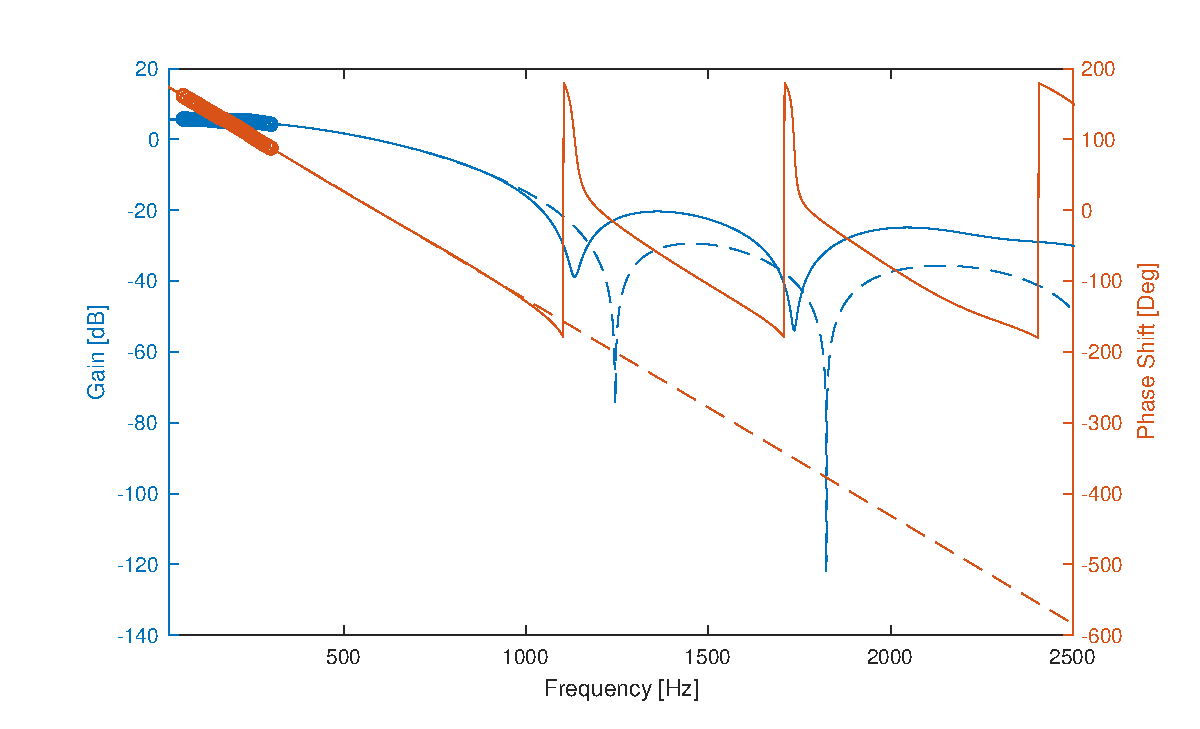
\includegraphics[width=1\textwidth]{filter_vs_reg.eps}
	\caption{The graph shows transfer function of the estimated impulse respond. The dashed line is transfer function that is needed for beam forming filter, where the blue line is the gain and the red line is the phase. The Solid line line is the transfer function of the estimated impulse response, where the blue line is the gain and the red line is the phase. All circle in the start of the graph is the actual optimized point.}
		\label{fig:filter_vs_reg}
\end{figure}

\begin{figure}[H]
	\centering
	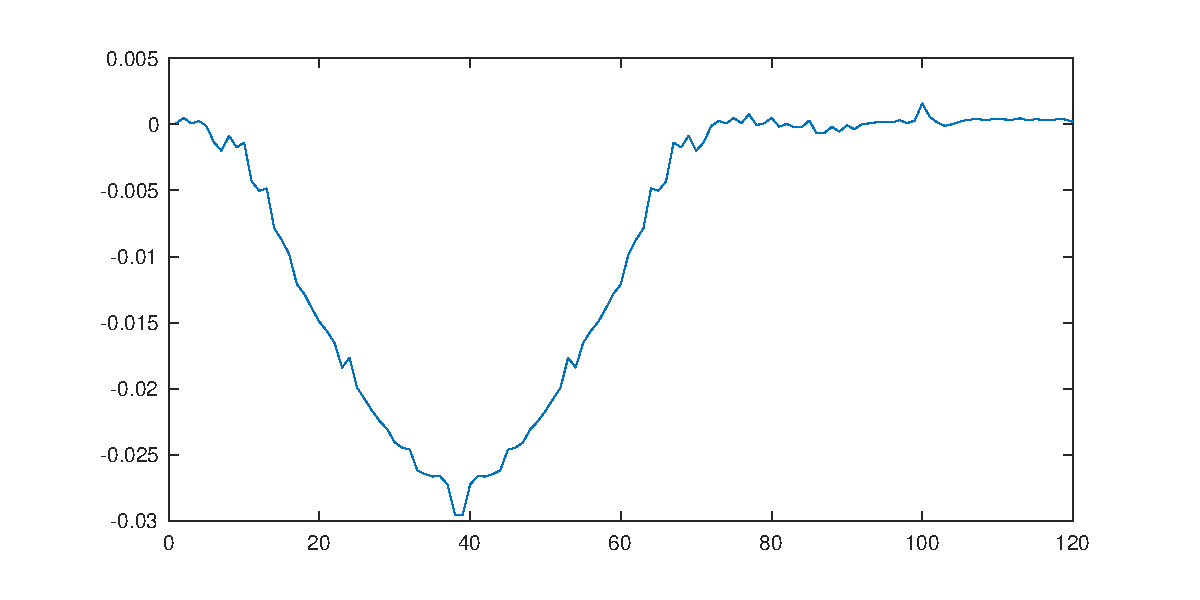
\includegraphics[width=1\textwidth]{filter_coefficient.eps}
	\caption{The graph shows the impulse respond where the mirrored version is added to the impulse respond}
		\label{fig:filter_coefficient}
\end{figure}

As it can be seen at \autoref{fig:ir_estimate_scaled} that the cut off is lowered and the gain is automatic raised to the wanted area. A closer look on the area of the frequency of interest in 


\begin{figure}[H]
\begin{subfigure}[c]{0.5\textwidth}
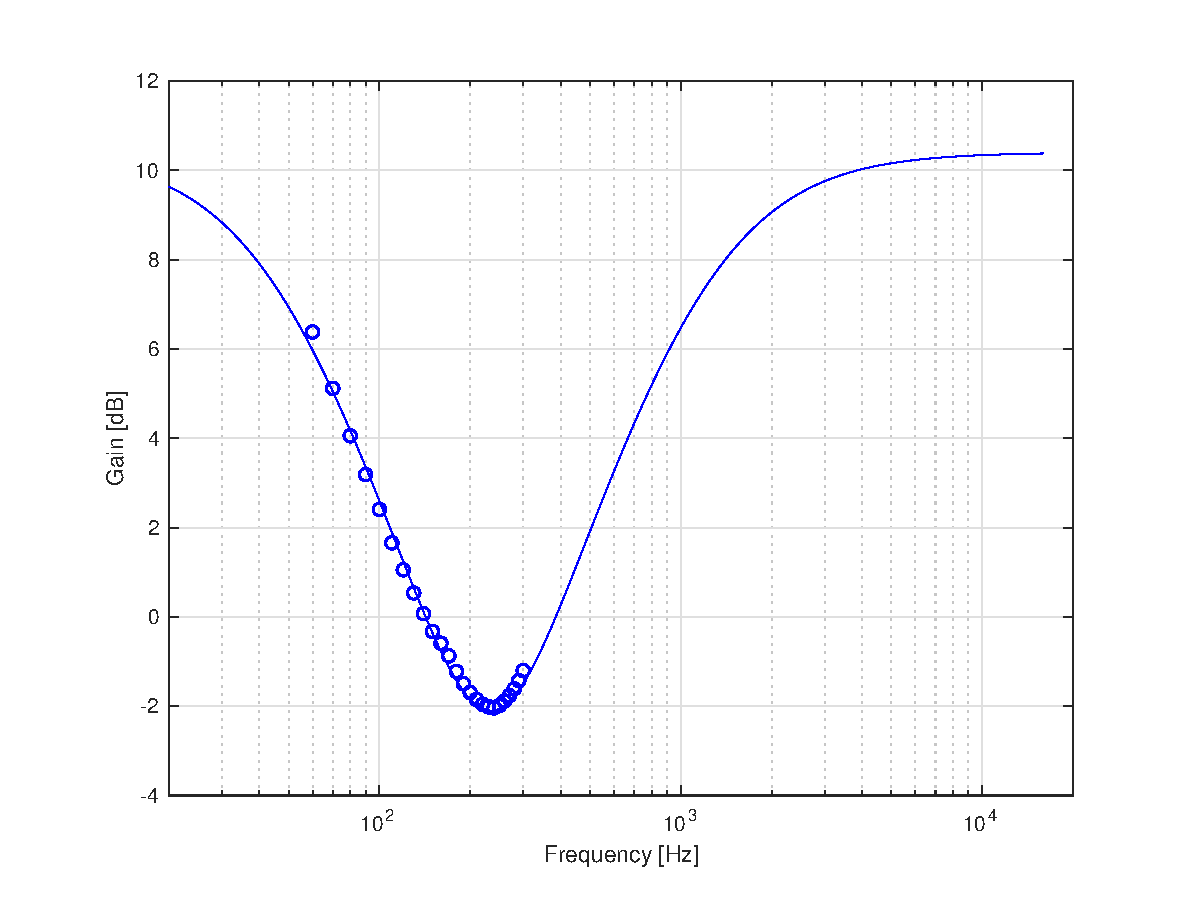
\includegraphics[width=0.85\textwidth]{opt_c_final.eps}
\subcaption{cost filter}
\label{fig:opt_res_a_finish}
\end{subfigure}
\begin{subfigure}[c]{0.5\textwidth}
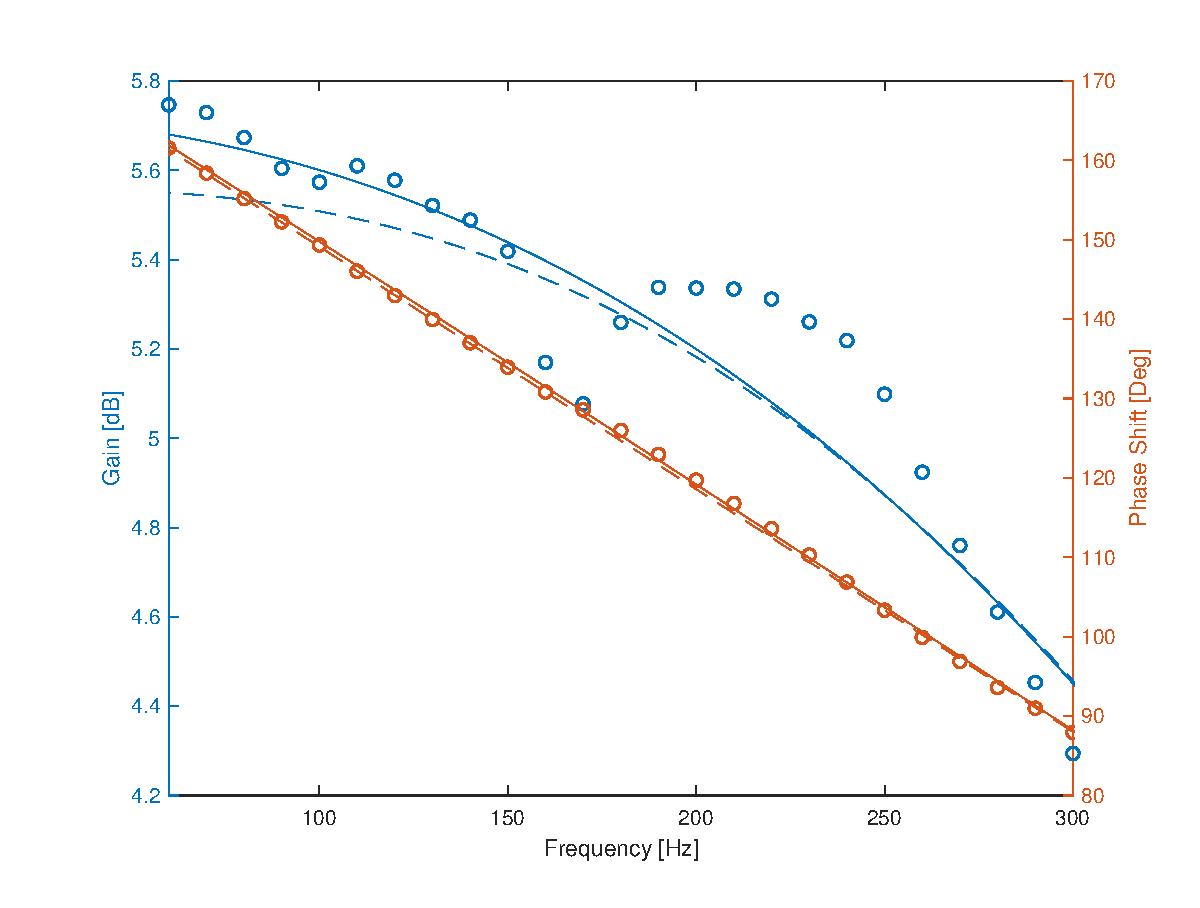
\includegraphics[width=0.95\textwidth]{filter_vs_data.eps}
\subcaption{Beamforming filter}
\label{fig:filter_vs_data_finish}
\end{subfigure}\\
\hspace{0.1\textheight}
\begin{subfigure}[c]{0.5\textwidth}
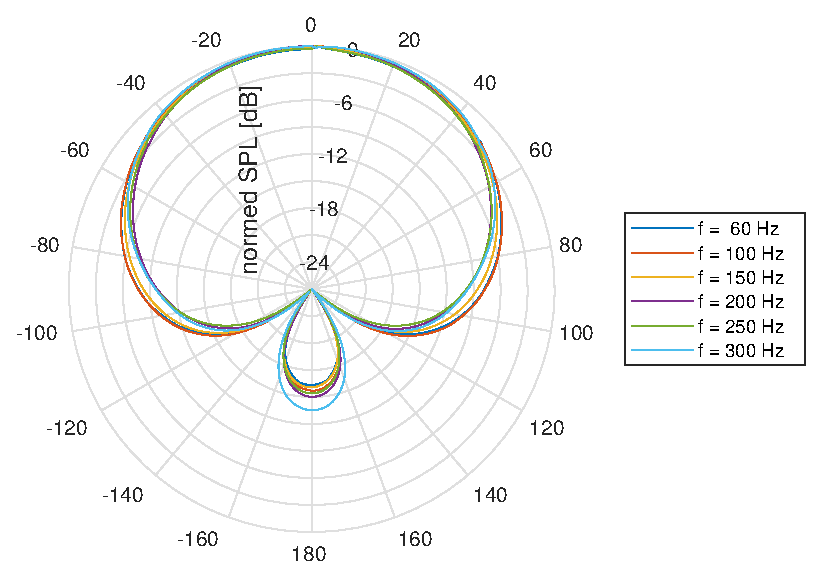
\includegraphics[width=0.95\textwidth]{opt_c.eps}
\subcaption{Directional characteristic, optimal}
\label{fig:opt_res_c_finish}
\end{subfigure}
\begin{subfigure}[c]{0.5\textwidth}
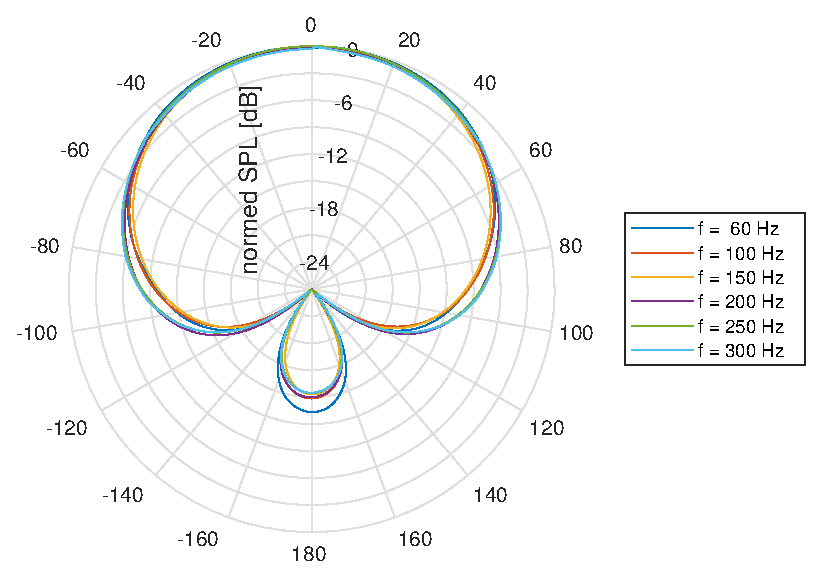
\includegraphics[width=0.95\textwidth]{polar_filtered.eps}
\subcaption{Directional characteristic, filtered}
\label{fig:polar_filtered_finish}
\end{subfigure}
\caption{Filter results, with pressure corrected cost filter, correction table based on Appendix \ref{ax:directional_2}, \textcolor{green3}{\texttt{Lx}}\,$=$\,\SI{0.4}{\meter}, \textcolor{green3}{\texttt{Ly}}\,$=\,$\SI{-0.4}{\meter}}
		\label{fig:opt_res_finish}
\end{figure}


\section{Conclusion}
It can be concluded that it is possible to design the cost filter as a band stop \gls{iir} filter and the beamforming filter as a low pass \gls{fir} filter. It can also be concluded that the filter does not change the beamforming significant, it accely change the  beamforming less than or equal \SI{1}{\decibel} for all frequency, both in the back and in the side of the polar plot \autoref{fig:opt_res_finish}.





